\documentclass[../thesis.tex]{subfiles}

\providecommand{\zcut}{z_\mathrm{{cut}}}
\providecommand{\LIPS}{\mathrm{LIPS}}
\providecommand{\cusp}{\mathrm{cusp}}
\providecommand{\mMDT}{\mathrm{mMDT}}

\providecommand{\arctanh}{\mathrm{arctanh}}
\providecommand{\Li}{\mathrm{Li}}

\providecommand{\cM}{\mathcal{M}}
\providecommand{\cL}{\mathcal{L}}
\providecommand{\cO}{\mathcal{O}}


\setlength{\parskip}{0pt}
%%
%% End Preamble
%%
%% The fun begins:
\begin{document}
	We would like to compute the soft function of Eq.~\ref{all-eq:soft function specific coords},
	\begin{equation}\label{app_soft-eq:soft function integral}
	\begin{aligned}
		S_R(\rho_s) &= \frac{\pi \alpha_s C_F \mu^{2\epsilon}}{\pi^{5/2} \Gamma(\frac{1}{2} - \epsilon)} \int dk_\perp d\phi_k d\eta_k \,k_\perp^{1 - 2\epsilon} \sin^{-2\epsilon} \phi_k \, \Theta(k_\perp)\Theta(\eta_k) \frac{2}{k_\perp^2} \\
		&\times \Bigg[ \Theta\qty(\sinh\eta_k - \cos\phi_k \cot\frac{\theta_g}{2}) \delta\qty(\rho_s - \frac{4k_\perp e^{-\eta_k}}{Q}) \\
		&\qquad+ \Theta\qty(\cos\phi_k \cot\frac{\theta_g}{2} - \sinh\eta_k) \\
		&\hspace{2cm}\times \delta\qty(\rho_s - \frac{4k_\perp}{Q}\qty[\cosh\eta_k - \cos\phi_k \sin\theta_g - \sinh\eta_k \cos\theta_g]) \Bigg] \\
		&\times \qty[1 - \Theta(\cos\theta_g - \tanh \eta_k)\Theta(\cot\theta_g - e^{\eta_k}\cos\phi_k)],
	\end{aligned}
	\end{equation}
	to a point where we can extract the anomalous dimension. The first step is to integrate out $k_\perp$, which can be done easily enough using the Dirac delta functions. The first transforms as
	\begin{equation}
		\delta\qty(\rho_s - \frac{4k_\perp e^{-\eta_k}}{Q}) = \frac{Q e^{\eta_k}}{4} \delta\qty(k_\perp - \frac{Q \rho_s e^{\eta_k}}{4}),
	\end{equation}
	while the second transforms as
	\begin{equation}
	\begin{aligned}
		\delta\Big(\rho_s - \frac{4 k_\perp}{Q}&\qty[\cosh\eta_k - \cos\phi_k\sin\theta_g - \sinh\eta_k\cos\theta_g]\Big) \\
		&= \frac{Q}{4\qty(\cosh\eta_k - \cos\phi_k\sin\theta_g - \sinh\eta_k\cos\theta_g)} \\
		&\qquad\times\delta\qty(k_\perp - \frac{Q \rho_s}{4\qty[\cosh\eta_k - \cos\phi_k\sin\theta_g - \sinh\eta_k\cos\theta_g]}).
	\end{aligned}
	\end{equation}
	Therefore, integrating out $k_\perp$ from Eq.~\ref{app_soft-eq:soft function integral}, we are left with
	\begin{equation}\label{app_soft-eq:soft integral without kperp}
	\begin{aligned}
		S_R(\rho_s) = \frac{2\pi\alpha_s C_F\mu^{2\epsilon}}{\pi^{5/2} \Gamma(\frac{1}{2} - \epsilon)} &\qty(\frac{Q}{4})^{-2\epsilon} \frac{1}{\rho_s^{1+2\epsilon}} \int d\phi_k d\eta_k\, \sin^{-2\epsilon}\phi_k \, \Theta(\eta_k) \\
		&\times \Bigg[ \Theta\qty(\sinh\eta_k - \cos\phi_k\cot\frac{\theta_g}{2})\,e^{-2\epsilon\eta_k} \\
			&\qquad+ \Theta\qty(\cos\phi_k\cot\frac{\theta_g}{2} - \sinh\eta_k)\\
			&\hspace{1cm}\times \qty(\frac{1}{\cosh\eta_k - \cos\phi_k\sin\theta_g - \sinh\eta_k\cos\theta_g})^{-2\epsilon}\Bigg] \\
			&\times \qty[1 - \Theta(\cos\theta_g - \tanh\eta_k)\,\Theta\qty(\cot\theta_g - e^{\eta_k}\cos\phi_k)].
	\end{aligned}
	\end{equation}
	Now, in order to extract the anomalous dimension, we need to determine, in Laplace space, the coefficient of the $2/\epsilon$ {\color{red}\textbf{[TODO: check factor of 2]}} term of the Laurent expansion of $S_R$ in $\epsilon$. Under a Laplace transformation taking $\rho_s \to \nu$, we have
	\begin{equation}
		\cL\qty{\frac{1}{\rho_s^{1 + 2\epsilon}}} = \nu^{2\epsilon} \Gamma(-2\epsilon) = -\frac{1}{2\epsilon} - \log\nu - \qty(\frac{\pi^2}{6} + \log^2\nu)\epsilon + \cO(\epsilon^2).
	\end{equation}
	This means that, in order to compute the anomalous dimension, we will need to keep terms through order $\cO(\epsilon^0)$ in the integral.

	To actually compute the integral, we will first make a sneaky simplification. Notice that, if we factor out $e^{-2\epsilon\eta_k}$,
	\begin{equation}
	\begin{aligned}
		&\Theta\qty(\sinh\eta_k - \cos\phi_k\cot\frac{\theta_g}{2})\,e^{-2\epsilon\eta_k} \\
			&\qquad+ \Theta\qty(\cos\phi_k\cot\frac{\theta_g}{2} - \sinh\eta_k)\, \qty(\frac{1}{\cosh\eta_k - \cos\phi_k\sin\theta_g - \sinh\eta_k\cos\theta_g})^{-2\epsilon} \\
		&= e^{-2\epsilon\eta_k} \Bigg[\Theta\qty(\sinh\eta_k - \cos\phi_k\cot\frac{\theta_g}{2}) \\
			&\qquad\qquad\qquad + \Theta\qty(\cos\phi_k\cot\frac{\theta_g}{2} - \sinh\eta_k)\, \qty(\frac{e^{-\eta_k}}{\cosh\eta_k - \cos\phi_k\sin\theta_g - \sinh\eta_k\cos\theta_g})^{-2\epsilon}\Bigg].
	\end{aligned}
	\end{equation}
	This converges as we send $\epsilon_k \to \infty$, so we can expand the term in brackets to find
	\begin{equation}
	\begin{aligned}
		\Theta&\qty(\sinh\eta_k - \cos\phi_k\cot\frac{\theta_g}{2}) \\
			&\quad + \Theta\qty(\cos\phi_k\cot\frac{\theta_g}{2} - \sinh\eta_k)\, \qty(\frac{e^{-\eta_k}}{\cosh\eta_k - \cos\phi_k\sin\theta_g - \sinh\eta_k\cos\theta_g})^{-2\epsilon} \\
			&= 1 + \cO(\epsilon).
	\end{aligned}
	\end{equation}
	We therefore find that
	\begin{equation}
	\begin{aligned}
		S_R(\rho_s) &= \frac{2\pi \alpha_s C_F \mu^{2\epsilon}}{\pi^{5/2} \Gamma(\frac{1}{2} - \epsilon)} \qty(\frac{Q}{4})^{-2\epsilon} \frac{1}{\rho_s^{1 + 2\epsilon}} \int d\phi_k d\eta_k \sin^{-2\epsilon}\phi_k \Theta(\eta_k) e^{-2\epsilon\eta_k} \\
			&\hspace{2cm}\times \qty[1 - \Theta(\cos\theta_g - \tanh\eta_k)\,\Theta\qty(\cot\theta_g - e^{\eta_k}\cos\phi_k)] + \cO(\epsilon^0).
	\end{aligned}
	\end{equation}
	For the first integral, we have (where $\phi_k$ ranges from $0$ to $\pi$)
	\begin{equation}
		\int d\phi_k d\eta_k \sin^{-2\epsilon} \phi_k \Theta(\eta_k) e^{-2\epsilon \eta_k} = \frac{1}{2\epsilon} \frac{\sqrt{\pi}\,\Gamma(\frac{1}{2} - \epsilon)}{\Gamma{1 - \epsilon}}.
	\end{equation}
	The second integral is not divergent in $\eta_k$ if we first set $\epsilon = 0$, so we can do that. Then we are left with
	\begin{equation}
	\begin{aligned}
		S_R(\rho_s) &= \frac{2\pi \alpha_s C_F \mu^{2\epsilon}}{\pi^{5/2} \Gamma(\frac{1}{2} - \epsilon)} \qty(\frac{Q}{4})^{-2\epsilon} \frac{1}{\rho_s^{1 + 2\epsilon}} \Bigg[ \frac{1}{2\epsilon} \frac{\sqrt{\pi}\,\Gamma(\frac{1}{2} - \epsilon)}{\Gamma(1 - \epsilon)}  \\
			&\hspace{2cm}- \int d\phi_k d\eta_k \Theta(\eta_k) \Theta(\cos\theta_g - \tanh\eta_k) \\
			&\hspace{6cm}\times \Theta\qty(\cot\theta_g - e^{\eta_k}\cos\phi_k) \Bigg] + \cO(\epsilon^0).
	\end{aligned}
	\end{equation}
	To evaluate the remaining integral, we need to establish our region of integration. We can simplify the bounds as
	\begin{equation}
	\begin{aligned}
		\Theta(\cos\theta_g - \tanh\eta_k)&\Theta\qty(\cot\theta_g - e^{\eta_k}\cos\phi_k) \\
		&= \Theta\qty(\frac{1}{1+\sec\theta_g} - \cos\phi_k)\Theta\qty(\cot\frac{\theta_g}{2} - e^{\eta_k}) \\
			&\qquad+ \Bigg[\Theta\qty(\cos\phi_k - \frac{1}{1+\sec\theta_g})\Theta(\cot\theta_g - \cos\phi_k)\\
			&\hspace{5cm} \times \Theta\qty(\cot\theta_g\sec\phi_k - e^{\eta_k}) \Bigg].
	\end{aligned}
	\end{equation}
	Now, because
	\begin{equation}
		\arcsec(1 + \sec\theta_g) < \frac{\pi}{2}
	\end{equation}
	for $0 < \theta_g < \pi/2$, we can split the first term up for positive and negative values of $\cos\phi_k$:
	\begin{equation}
		\Theta\qty(\frac{1}{1+\sec\theta_g} - \cos\phi_k) = \Theta\qty(\frac{\pi}{2} - \phi_k)\Theta\qty(\sec\phi_k - 1 - \sec\theta_g) + \Theta\qty(\phi_k - \frac{\pi}{2}).
	\end{equation}
	Then evaluating the first part of the integral yields
	\begin{equation}
	\begin{aligned}
		\int d\phi_k d\eta_k &\Theta(\eta_k) \qty[\Theta\qty(\frac{\pi}{2} - \phi_k)\Theta\qty(\sec\phi_k - 1 - \sec\theta_g) + \Theta\qty(\phi_k - \frac{\pi}{2})]\Theta\qty(\cot\frac{\theta_g}{2} - e^{\eta_k}) \\
		&= \qty[\pi - \arcsec(1 + \sec\theta_g)] \log(\cot\frac{\theta_g}{2}).
	\end{aligned}
	\end{equation}
	
	The second part is a little more complicated. We can first integrate in $\eta_k$ to find
	\begin{equation}\label{app_soft-eq:integral after eta}
	\begin{aligned}
		\int &d\phi_k d\eta_k \Theta(\eta_k)\Theta\qty(\cos\phi_k - \frac{1}{1+\sec\theta_g})\Theta(\cot\theta_g - \cos\phi_k) \Theta\qty(\cot\theta_g\sec\phi_k - e^{\eta_k}) \\
		&\hspace{1.25cm}= \int d\phi_k \Theta\qty(\cos\phi_k - \frac{1}{1+\sec\theta_g})\Theta(\cot\theta_g - \cos\phi_k) \log(\cot\theta_g \sec\phi_k ).
	\end{aligned}
	\end{equation}
	To solve the remaining integral, first notice that
	\begin{equation}
		\cot\theta_g > 1 \implies \cot\theta_g > \cos\phi_k
	\end{equation}
	for $0 < \theta_g < \pi/4$. Therefore,
	\begin{equation}\label{app_soft-eq:pi/4 split}
		\Theta(\cot\theta_g - \cos\phi_k) = \Theta\qty(\frac{\pi}{4} - \theta_g) + \Theta\qty(\theta_g - \frac{\pi}{4})\Theta(\cot\theta_g - \cos\phi_k).
	\end{equation}
	Now that we have established the bounds, we can evaluate the indefinite integral:
	\begin{equation}\label{app_soft-eq:indefinite log integral}
		\int d\phi_k \log(\cot\theta_g \sec\phi_k ) = \frac{i \phi_k^2}{2} + \phi_k \log(2\cot\theta_g) - \frac{i}{2}\Li_2\qty(-e^{2i\phi_k}),
	\end{equation}
	where $\Li_2(x)$ is the dilogarithm function. This function is explored in Appendix \ref{app:dilogarithm}. From Eq.~\ref{app_dilog-eq:dilog exponential identity}, we have
	\begin{equation}
		\frac{i}{2}\Li_2\qty(-e^{2i\phi_k}) = -\frac{i \pi^2}{24} + \frac{i\phi_k^2}{2} - \frac{i}{4}\qty[\Li_2\qty(-e^{-2i\phi_k}) - \Li_2\qty(-e^{2i\phi_k})].
	\end{equation}
	Then Eq.~\ref{app_soft-eq:indefinite log integral} becomes
	\begin{equation}\label{app_soft-eq:indefinite log integral simplified}
		\int d\phi_k \log(\cot\theta_g \sec\phi_k ) = \phi_k \log(2\cot\theta_g) + \frac{i}{4}\qty[\Li_2\qty(-e^{-2i\phi_k}) - \Li_2\qty(-e^{2i\phi_k})] + \frac{i\pi^2}{24}.
	\end{equation}
	The imaginary part of this integral is manifestly a constant, $i\pi^2/24$, and therefore drops out when we perform a definite integral. Now notice that
	\begin{equation}
		\arccos\qty(\frac{1}{1 + \sec\theta_g}) = \arcsec(1 + \sec\theta_g).
	\end{equation}
	Thus, we can combine Eqs.~\ref{app_soft-eq:integral after eta}, \ref{app_soft-eq:pi/4 split}, and \ref{app_soft-eq:indefinite log integral simplified} to find
	\begin{equation}
	\begin{aligned}
		\int d\phi_k &\Theta\qty(\cos\phi_k - \frac{1}{1+\sec\theta_g})\Theta(\cot\theta_g - \cos\phi_k) \log(\cot\theta_g \sec\phi_k ) \\
		&= \arcsec\qty(1 + \sec\theta_g) \log(2\cot\theta_g) + \frac{i}{4}\Big [\Li_2\qty(-e^{-2i\arcsec\qty(1 + \sec\theta_g)}) \\
			&\hspace{7.75cm}- \Li_2\qty(-e^{2i\arcsec\qty(1 + \sec\theta_g)}) \Big] \\
		&\qquad- \Theta\qty(\theta_g - \frac{\pi}{4})\Bigg[ \arccos\cot\theta_g \log(2\cot\theta_g) \\
			&\hspace{3.75cm}+ \frac{i}{4}\qty[\Li_2\qty(-e^{-2i\arccos\cot\theta_g}) - \Li_2\qty(-e^{2i\arccos\cot\theta_g})] \Bigg].
	\end{aligned}
	\end{equation}
	We can therefore conclude that the full soft function through order $\cO(\epsilon^{-1})$ is
	\begin{equation}\label{app_soft-eq:full soft function}
	\boxed{
	\begin{aligned}
		S_R(\rho_s) &= \frac{2\pi\alpha_s C_F\mu^{2\epsilon}}{\pi^{5/2} \Gamma(\frac{1}{2} - \epsilon)}\qty(\frac{Q}{4})^{-2\epsilon} \frac{1}{\rho_s^{1 + 2\epsilon}} \\
			&\qquad\times \Bigg[\frac{1}{2\epsilon}\frac{\sqrt{\pi} \, \Gamma(\frac{1}{2} - \epsilon)}{\Gamma(1 - \epsilon)} - \qty[\pi - \arcsec(1 + \sec\theta_g)]\log\cot\frac{\theta_g}{2} \\
			&\qquad\qquad - \arcsec\qty(1 + \sec\theta_g) \log(2\cot\theta_g) \\
			&\qquad\qquad - \frac{i}{4}\qty[\Li_2\qty(-e^{-2i\arcsec\qty(1 + \sec\theta_g)}) - \Li_2\qty(-e^{2i\arcsec\qty(1 + \sec\theta_g)})] \\
			&\qquad\qquad+ \Theta\qty(\theta_g - \frac{\pi}{4})\Bigg[ \arccos\cot\theta_g \log(2\cot\theta_g) \\
			&\hspace{3cm}+ \frac{i}{4}\qty[\Li_2\qty(-e^{-2i\arccos\cot\theta_g}) - \Li_2\qty(-e^{2i\arccos\cot\theta_g})] \Bigg] \Bigg] + \cO(\epsilon^0).
	\end{aligned}
	}
	\end{equation}

	This has been a long calculation, and it would be nice to confirm that we did it right. We can compare our analytic result to numeric results after first fixing the values of the constants. Let $Q = 91.2$ \si{\giga\electronvolt} (the mass of the $Z$ boson), at which $\alpha_s = 0.118$ \cite{particle_data_group_review_2020}. Then take $C_F = 4/3$, and arbitrarily take $\mu = 10$ \si{\giga\electronvolt} and $\rho_s = 0.1$. Finally, since our analytic result is only accurate through order $\cO(\epsilon^{-1})$, we should take $\epsilon$ to be small so that higher-order corrections are small. Thus, let us take $\epsilon = 0.0001$. The result is displayed in Fig.~\ref{app_soft-fig:soft function numerics}. There is good agreement between the numerical result and the analytic one, which helps us feel confident that we performed the integral correctly.
	\begin{figure}
	\begin{center}
		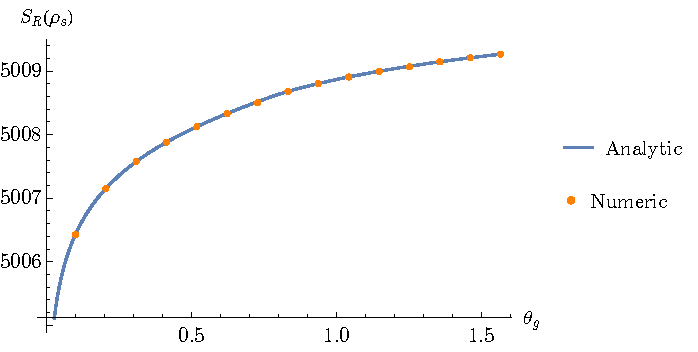
\includegraphics[width=0.9\textwidth]{figures/full_eps_0.0001.pdf}

		\caption{\label{app_soft-fig:soft function numerics}Analytic (blue curve) and numeric (orange dots) results for the soft function $S_R(\rho_s)$. The analytic curve is from Eq.~\ref{app_soft-eq:full soft function}, while the numeric result comes from evaluating Eq.~\ref{app_soft-eq:soft integral without kperp}. Constants are fixed to values described in the text.}
	\end{center}
	\end{figure}
\end{document}
